% Chapter 4 - Extensión de una aplicación RIA

\chapter{Extensi\'{o}n de una aplicaci\'{o}n RIA} % Chapter title

\label{ch:ria_extension} 

% ### Introducción de capítulo
El concepto, para una aplicación web como las que aquí se referencian, es el de \emph{Rich Internet Application} (RIA para resumir), estas aplicaciones poseen un conjunto de características que las distinguen de los ``sitios web'' o ``paginas web'' y de las aplicaciones de escritorio. 

La industria ha evolucionado en los últimos años hacia aplicaciones que pueden catalogarse como RIA's; aplicaciones web con una gran cantidad de lógica de negocio del lado del cliente y con alta atención en la experiencia del usuario. Algunos ejemplos son, Facebook, Gmail, Twitter, dentro del aplicaciones sociales; Rdio, Beats, como aplicaciones multimedia; BBC y NYTimes entre aplicaciones informativas. Estas compañías han impulsado diferentes técnicas y herramientas para el desarrollo de aplicaciones web modernas. 

Esta información será usada en este capítulo como contexto para entender la forma de encastrar la plataforma propuesta con las aplicaciones web contemporáneas.

\section{Aplicaciones RIA} \label{sec:extension_ria_intro}

Las denominadas \emph{aplicaciones web ricas} o RIAs se ubican, en una posible linea de tiempo histórica, como paso siguiente a los sitios web o paginas web pertenecientes a la \emph{web 1.0}. Son parte del cambio que implicó a la denominada \emph{web 2.0} y fueron evolucionando buscando algunos objetivos determinados que esta tendencia demandaba y que las distinguía de las aplicaciones web pertenecientes a la era ``1.0'', según \citet{Farrell2007}. 

En este marco histórico, el desarrollo busca centrarse en el usuario a través de la creación de experiencias e interacción mas ricas. La arquitectura de las aplicaciones \emph{web 1.0} estaba demasiado limitada por el paradigma cliente-servidor, donde el cliente era un simple consumidor de cada pagina de hipertexto que el servidor le generaba, esto presenta un sincronismo duro que afectaba fuertemente las capacidades de interacción.

En \citet{Duhl2003}, se definen los siguientes problemas tradicionales de las aplicaciones web pertenecientes a la época ``1.0'':
\begin{itemize}
\item Procesos complejos.
\item Dificultad en en el acceso y tratamiento de datos (ausencia de capacidades exploratorias).
\item Ausencia de capacidades de configuración y previsualización de objetos.
\item Bajo feedback (altamente fragmentado).
\end{itemize}
De acuerdo a  \citet{Fraternali2010}, las aplicaciones RIA representan una solución a estas limitaciones y/o problemas, ya que permiten construir aplicaciones con las siguientes características:
\begin{itemize}
\item Posibilidad de mantener datos en ambos extremos (cliente, servidor).
\item Esquema de lógica de negocios distribuida entre cliente servidor, con la posibilidad de balancear la carga completamente servidor, completamente cliente o mixto.
\item Igualdad en la capacidad de iniciar la conversación, tanto por parte del cliente como del servidor.
\end{itemize}

Estas capacidades permiten enriquecer la experiencia de uso de la aplicación web, haciéndola similar o incluso mejor que la contra-parte de escritorio. Particularmente, se destaca las mejoras que generan las RIA sobre el ultimo punto, el feedback. Estas aplicaciones se basan en el asincronismo en la carga y actualización de componentes, permitiendo así ``independizarlos'' en la información que representan mientras siguen siendo partes de un aplicativo superior. Por ejemplo, esto puede notarse en cualquier aplicación web que permita elegir qué elementos cargar de una lista sin refrescar toda la página y a la vez permitiendo interactuar con este, recientemente agregado, componente. Este estilo de aplicación es conocido como \emph{Single Page Application} (SPA) o aplicación de una sola pagina.

Finalmente, es menester tener en cuenta que las características previamente listadas han mejorado notablemente en los últimos años. Un ejemplo de esto es el nuevo estándar HTML5, que no representa una tecnología particular si no mas bien un conjunto de tecnologías (CSS, HTML y JS). Estas herramientas en conjunto dan muestra de progresos importantes en la presentación, estructura y lógica de la aplicación web que se va a ejecutar del lado del cliente.

\section{Conexión con RIA} \label{sec:extension_ria_conexion}

La definición de una aplicación rica (RIA) no esta ligada a un lenguaje en particular, por lo tanto pueden existir diferentes implementaciones de las mismas en el mercado, sin embargo, de acuerdo al trabajo de \citet{Bozzon2006} es posible clasificarlas en cuatro tipos:

\begin{itemize}
\item \emph{Scripting-based} o basadas en scripting; ~estas aplicaciones son de las mas populares y están compuestas en su mayoría de JavaScript y técnicas como AJAX.
\item \emph{Plugin-based} o basadas en plugines; ~este tipo de aplicación se apoya en alguna plataforma y ambiente particular, \eg~ Flash, Flex. 
\item \emph{Browser-based} o basadas en algún browser; ~aplicaciones de este estilo corren dentro del ambiente de algún browser especifico, usualmente como extensiones del mismo y aprovechan a su vez APIs que éste define.
\item \emph{Web-based desktop technologies}; ~son aplicaciones que pueden ser descargadas en primer medida desde la web, pero tienen requerimientos extras particulares (\ie ~dependencias) y corren fuera del browser.
\end{itemize}

La solución propuesta en este trabajo de tesis, apunta a operar con aplicaciones RIA del tipo \emph{scripting-based}, ya que se han convertido en las mas populares y con mas soport \emph{open-source}, aunque hay que destacar que la plataforma es agnóstica a la caracterización de la aplicación, esto implica que no posee requerimientos fuertes sobre donde será usada. Habiendo mencionado esto, es probable que sea necesario el desarrollo o uso de algún \emph{wrapper} o adaptador especifico para poder correr en un ambiente determinado como puede ser el de una solución estilo \emph{plugin-based}, aunque este desarrollo extra debería ser mínimo y acotado.

\subsection{Conexión con RIA y MDD} \label{sec:extension_ria_mdd_conexion}

El desarrollo dirigido por modelos o \emph{model-driven development} (resumido como MDD), es una técnica bastante popular para el desarrollo de RIAs. Uno de los objetivos en el uso de MDD es minimizar y controlar la complejidad inherente que posee una aplicación web rica. 

Muchas metodologías se han propuesto para modelar RIAs \citep{wright2008requirements} \citep{preciado2005necessity}, la mayoría extiende estrategias de modelado para aplicaciones de la era ``1.0''. Esto ha generado demasiada fragmentación que dejo en evidencia, al menos, las dificultades para modelar aplicaciones de este estilo. 

WebML\citep{omg:webml} es una de estas técnicas, que recientemente ha sido reformateada en el nuevo estándar del \citet{omg:omg}, como IFML \citep{omg:ifml} o \emph{Interaction Flow Modeling Language}. 

Si bien la plataforma \emph{Plusultra}, como ya se ha mencionado, es agnóstica al tipo de RIA desarrollada, ésta añade capacidades de interacción nuevas al conjunto soportado por las aplicaciones web. Estas nuevas capacidades de interacción pueden ser modeladas como \emph{eventos} dentro del sistema. 
Es decir, estas formas de interacción pueden modelarse, dentro de una metodología de desarrollo basado en modelos, usando a su vez IFML para contemplar la interacción; como nuevos \emph{eventos} añadidos al contexto de la aplicación.

\subsection{Conexión con RIA y MDD: Ejemplo}

Si bien no es el objetivo principal del presente trabajo explayarse sobre una metodología de desarrollo particular, parece importante destacar al menos con un pequeño y concreto ejemplo la posibilidad de utilizar un estándar para el modelado de la aplicación desde el \emph{front-end}. 

Para ello, se ha considerado la metodología IFML para modelar un posible flujo de interacción de la aplicación ejemplo, \emph{Shapes}. En la figura \ref{fig:extension_ifml_example}, se muestra el modelado de acciones relacionadas a una fisión. En este momento, el sistema ha detectado que se ha producido una fisión , la cual es replicada a través de \emph{Gyes} y \emph{Plusultra} y se han ejecutado las acciones correspondientes asociadas a los eventos, en este caso, de interpretación y fisión.

% FIGURA DE MODELADO IFML - shapes app
\begin{center}
  \begin{figure}[h]
    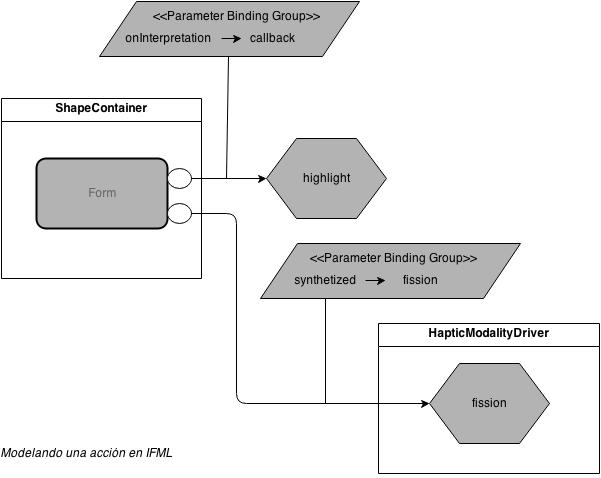
\includegraphics[scale=1,width=\textwidth]{gfx/ifml_example}
    \caption{Modelado de acciones en Shapes App.}
    \label{fig:extension_ifml_example}
  \end{figure}
\end{center}

\section{Aplicaciones Web en la Industria} \label{sec:extension_industria_intro}

La industria ha sido participe en la mencionada ``revolución 2.0''. Negocios como \emph{amazon} crecen considerablemente en esta época y generan necesidades nuevas, lo que motiva a la competencia a imitarlas o superarlas. Con el objetivo de mejorar cualitativamente las aplicaciones desarrolladas y las nuevas por crear, la industria comenzó a generar sus propias herramientas, muchas de ellas \emph{open source}, lo que permitió que otros las usaran, mejorando de esta manera la calidad general del ecosistema.

En este contexto es donde surgen librerías troncales como Backbone.js \citep{ind:backbone}, en el 2010, la cual esta desarrollada íntegramente en JavaScript y ofrece directamente al desarrollador abstracciones para modelos, vistas y controladores desde el lado del cliente, asumiendo del lado del servidor, una API REST. Una librería de este estilo, con un conjunto de dependencias mínimo colaboro directamente con el desarrollo de aplicaciones web ricas, con gran parte de lógica del lado del cliente, capaces de manejar y disparar \emph{in-situ} eventos generados por la misma aplicación o por algún \emph{third-party}. De esta forma se produce un traslado masivo del patrón MVC relacionado tradicionalmente al \emph{backend}, hacia el \emph{frontend}. 

Unos años mas tarde, aparecen nuevas herramientas mas robustas; del tipo \emph{frameworks}, nuevamente desarrolladas en JavaScript. El objetivo de estos frameworks es el mismo, ayudar al desarrollador a generar, mantener y permitir escalar una aplicación ``del lado del cliente'', usualmente siguiendo el estilo de backbone.js, consumiendo datos desde algún servicio que se encuentre corriendo del lado del servidor. 

Entre estos frameworks, se pueden destacar Angular.js de \citep{ind:angular} y Ember.js \citep{ind:ember}. Nuevamente, estas herramientas son \emph{open source} y tienen gran soporte por parte de sus respectivas comunidades, lo que permite retro-alimentar el ecosistema de aplicaciones ricas, haciéndolas perdurar en el tiempo.

Dentro de la industria no hay que dejar de lado a los desarrolladores de navegadores. Grandes empresas como Google, Apple y la fundación Mozilla contribuyen a la mejora de este escenario a través del desarrollo de navegadores que implementen los estándares de la W3C. Esto posibilita el acceso a nuevas capacidades, como por ejemplo la API para WebRTC, la tecnología que permite acceder a recursos tales como la cámara o el micrófono y compartirlos por internet. Hay que tener en cuenta la relación existente entre la implementación de los estándares y estas grandes compañías, ya que usualmente desarrolladores pertenecientes a las mismas participan en los comités donde se definen estas nuevas APIs. 

\section{Conexión con la Industria} \label{sec:extension_industria_conexion}

Similar al caso anterior, la relación entre las aplicaciones web modernas que se pueden desarrollar utilizando las herramientas que brinda la industria y la plataforma propuesta no implica una dependencia entre ambas. 

La plataforma puede ser consumida desde el contexto de una aplicación web a través del uso de una librería provista, \emph{Gyes}. Dicha librería, encapsula una API de acceso a la plataforma y es vista desde la aplicación como una dependencia mas. 

\marginpar{La definición actual JavaScript (ES2015) no soporta un concepto de modulo nativo, para suplir esta carencia la industria ha desarrollado varias técnicas que involucran \emph{wrappers} que permiten modularizar y cargar bajo demanda. Estas técnicas son CommonJS (CJS), AMD y UMD. CommonJS ha sido implementado en Node.js, AMD fue una de las primeras especificaciones para componentizar desde el lado del cliente. CJS y AMD no son compatibles entre si; es por esto que nace UMD, un patrón que envuelve tanto código CJS y/o AMD y lo hace interoperable.}

\emph{Gyes} puede esta escrita usando el formato de módulo CommonJS \citep{ind:commonjsmodules} compatible con Node.js. Esto permitió modularizar las distintas dependencias internas de la aplicación. Ya que este formato no es soportado por los navegadores, se utiliza un proceso de construcción que genera un archivo único que representa la dependencia antes mencionada y que es compatible con los navegadores, gracias al uso del patrón UMD\footnote{Para mas información ver: https://github.com/umdjs/umd}. A su vez, esta dependencia puede encapsularse dentro del formato AMD para ser gestionada mediante otras herramientas como requirejs \citep{ind:requirejsmodules}, por ejemplo. 

En un futuro seria interesante portar \emph{Gyes} al sistema de módulos estándar propuesto para JavaScript, pero el mismo hasta el momento no se encuentra soportado por los navegadores corrientes.

\section{Resumen del Capítulo} \label{sec:extension_conclusion}

Se ha especificado el contexto de aplicación web en el cual la plataforma puede insertarse. 

Se ha puesto énfasis en analizar este contexto desde dos aristas, el ámbito académico y la industria. De esta forma es mas claro ver como se puede utilizar la herramienta desarrollada y como encaja en el escenario actual y en un entorno de producción.

En el siguiente capítulo se mostrará de forma integral el uso de la plataforma por medio del desarrollo de una aplicación web que servirá también como modo de \emph{validación por implementación} para la plataforma.